\documentclass{article}
\usepackage[utf8]{inputenc}
\PassOptionsToPackage{hyphens}{url}\usepackage{hyperref}
\usepackage{amsmath}
\usepackage{csvsimple}
\usepackage{subcaption}
\usepackage{adjustbox}
\usepackage[T1]{fontenc}
\usepackage{grffile}
\usepackage[margin=1in]{geometry}
\usepackage{appendix}
\usepackage{xcolor}
\usepackage[nottoc]{tocbibind}
\usepackage[section]{placeins}
%\usepackage{subfig}
\usepackage{paralist}
\usepackage[capitalise,nameinlink,noabbrev]{cleveref}
\usepackage{bm}
\usepackage{hyperref}

\hypersetup{
    colorlinks=true,
    linkcolor=blue,
    filecolor=magenta,      
    urlcolor=cyan,
}

\setlength{\parindent}{5ex}
\setlength{\parskip}{1ex}
\def\LukeDoStates{1}

\makeatletter
\csvset{
  autotabulartop/.style={
    file=#1,
    after head=\csv@pretable\begin{tabular}[t]{|*{\csv@columncount}{l|}}\csv@tablehead,
    table head=\hline\csvlinetotablerow\\\hline,
    late after line=\\,
    table foot=\\\hline,
    late after last line=\csv@tablefoot\end{tabular}\csv@posttable,
    command=\csvlinetotablerow}
}
\makeatother
\newcommand{\csvautotabulartop}[2][]{\csvloop{autotabulartop={#2},#1}}


\newcommand{\AddLukeFigure}[3]{
\begin{figure}
  \centering
  \begin{subfigure}{0.48\linewidth}
    \includegraphics[width=\linewidth]{luke/#1_#2_linear.pdf}
    \caption{Linear Scale}
  \end{subfigure}
  \begin{subfigure}{0.48\linewidth}
    \includegraphics[width=\linewidth]{luke/#1_#2_log.pdf}
    \caption{Log Scale}
  \end{subfigure}

  \begin{subfigure}{0.96\linewidth}
    \includegraphics[width=\linewidth]{luke/#1_#2_legend.pdf}
  \end{subfigure}
    \caption{Doubling and cumulative cases (#3)}
    \label{fig:doublings_#1_#2}
\end{figure}

\begin{figure}
  \centering
  \includegraphics[width=.6\linewidth]{luke/#1_#2_test.pdf}
  \caption{Histogram and box plot (#3)}
  \label{fig:test_#1_#2}
\end{figure}
}

\title{ISYE 6739 Project Final Report}
%For tomorrow:
%For each person
%    Have raw data, analysis, implications and future work
%    Have visuals for presentation complete
%    If have time do writeup audio part

\author{Lechen Yu, Sara Miller, Matt Gudorf, Luke Erlandson}
%Order: Lechen Matt Luke Sara
\date{Spring 2020}

\begin{document}

\maketitle

%\section*{Abstract}
\begin{abstract}

This work investigates the geographic and temporal transmission of the 2019 novel coronavirus. A variety of statistics tools were used to draw inferences on this highly-dynamic problem. %Add Lechen's Stuff %Add Matt's Stuff 
Social distancing, quarantines, stay-at-home orders and other mandates have slowed the spread of COVID-19 throughout the world. These practices come with their own costs, however, in regards to mental health, unemployment, education, etc. Because the situation is in a constant state of change, it is important to identify the most effective measures because they might need to be reenacted upon the emergence of a second wave of proliferation.
%Luke's Stuff
We preform an investigation on the doubling rate of the infection rate by country, both as a distribution and looking at individual countries.
Finally, a literature review of peer-reviewed medical journals was performed to compile a data set with published estimates of the basic reproduction number ($R_0$). From these published estimates, a meta-analysis was performed to answer the following question: is $R_0$ for COVID-19 in China decreasing with time? A simple linear regression analysis showed no significant correlation between the dates of the studies and their resulting estimates for $R_0$. Therefore, we conclude that more time must pass before the relationship between $R_0$ and time can be gleaned from simple linear regression. An online version of our presentation is available via \href{https://docs.google.com/presentation/d/17ZegWwXkD2-FEV-3EgUg825KnwtbHrZZuWgpTryxcOs/edit?usp=sharing}{Google Slides}.

\end{abstract}
\tableofcontents

\section{Background and Justification}

The 2019 novel coronavirus (COVID-19) has already resulted in more deaths than severe acute respiratory syndrome (SARS) and Middle East respiratory syndrome (MERS) combined, so understanding the transmission dynamics of this outbreak is critical to informing the public health approach \cite{1}. The current report focuses on the growth patterns associated with COVID-19, as indicated by the number of confirmed cases and number of deaths. To understand this phenomenon, we consider the effect of weather and geographic location, estimates of the virus' reproduction number obtained from medical journals, the doubling time between countries, and the impact of self-isolation measures. 

\section{Description of Raw Data}
%1-2 Paragraphs each

%Lechen's Data Description
The COVID-19 Open Research dataset~\cite{covid19weather} is used in the study of COVID-19's spread. This dataset consists of there parts:
\begin{inparaenum}[a)]
    \item COVID-19 confirmed cases and fatalities group by regions (states), 
    \item geography data (e.g., latitude and longitude), and
    \item 9 categories of weather data imported from NOAA GSOD dataset~\cite{weatherdata}.
\end{inparaenum}
It records the confirmed cases from \date{2020-01-22} through \date{2020-04-11}. To reason about the spread of COVID-19 in China, we analyzed the average growth rate and daily growth rate in each region, via a number of statistical methods. The average growth rate and series of daily growth rates are calculated based on the number of confirmed cases. The normality of daily growth rates is tested by D'Agostino's K-squared test~\cite{normaltest}. For each region's average growth rate, two analysis was conducted:
\begin{inparaenum}[a)]
    \item using covariance to analyze the relationship between the growth rate and distance to Hubei (the outbreak province of COVID-19), and 
    \item using ANOVA to compare the growth rates in distinct environments.
\end{inparaenum}
Through these analysis, we try to figure out potential factors that have a positive/negative effect on the spread of COVID-19.


%Matt's Data Description
Three datasets were used in the test of the effects of country and government mandates. These three datasets included
data on the dates of different quarantine measures per country \cite{govtresponse},  the time series data for the case numbers \cite{owid} and the time series data on the number of tests \cite{find}. These datasets are quite inconsistent due to differences in reaction to the pandemic and the inconsistency of reporting. This manifests as irregular time-series, in terms of the dates on which they are defined, as well as missing values. 
Because of this, a number of actions which may or may not be heavy handed needed to be employed.  
These actions accounted for the following: differences in time series ranges, missing values, quarantine measures which occur before the first recorded case in a country, dissimilar quarantine measures taken and differences in the countries whose data was recorded. 
To make the data uniform, the time series were normalized to be from December 31st 2019 to April 20th, 2020. The end date was simply because one of the data sets has not been updated in the past week. The original missing values and those created by this normalization were handled by using linear interpolation on the interior of the time series and linear extrapolation for the beginning of the time series. This is only applied at the very beginning of each countries time series (if values are missing) typically when the cases number is very small or even equal to 1. Therefore, I believe this action is justified by using linear expansion of exponential growth. After the time series were made uniform, the specific government responses to investigate
were chosen by how widespread their adoption was. The countries were determined by taking the intersection of all countries present in the three data sets.

The doubling time of the virus is an important number as it provides an indication of how quickly the spread is happening. It is relatively simple to determine from cumulative data, directly arising from the data rather than requiring additional analysis.
However, it does not provide specific or individual information, and can vary greatly depending on the timescale.
To calculate and analyze the doubling of COVID-19, we looked at a dataset provided by Johns Hopkins \cite{john_hopkins}, which provides information of many different regions on a day by day basis. 
These regions are either global regions, consisting of countries or large regions.
\if\LukeDoStates1
Additionally, data for the United States in the format was used.
\fi
This data is updated daily, as such we have data from 2020-01-22 through \input{luke/end_date.csv}
The data consists of a CSV file where each row corresponds with a region, there are a few columns of meta-data, followed by the remaining columns, one for each day since 2020-01-22, which contain the number of cumulative confirmed cases on a given day.
Additionally, we referenced the calculated doubling time from \cite{systemic_review}, \cite{high_contagiousness}, to compare our results to.


The basic reproduction number, $R_0$, is used by epidemiologists to quantify the intensity of an infectious disease. A disease’s $R_0$ is defined as the average number of people who will contract a disease from one contagious person. Thus, an accurate estimate of $R_0$ is instrumental to characterizing the transmission of COVID-19. An $R_0$ $>$ 0 indicates that the number of infected people is likely to increase, whereas an $R_0$ $<$ 0 indicated that the transmission of the disease is likely to die out. Therefore, the higher a disease’s $R_0$, the greater the risk to a population. A literature review of peer-reviewed medical journals was conducted to compile a data set of estimates for $R_0$ for COVID-19 in China. A total of 32 estimates for $R_0$, along with the corresponding 95\% confidence intervals and study dates, are provided in Appendix A. In the literature, a confidence level of 95\% was found to be the standard for discussions involving $R_0$. The "Study Date" column in Appendix A refers to the cutoff date for the number of COVID-19 confirmed cases that was used in each study. Some researchers used different mathematical models to develop multiple estimates of $R_0$ and each of those estimates was included as separate data points. Due to the overlap of data sets, researchers, and mathematical approaches to estimating $R_0$, this data is not independent.

\section{Statistical Analyses}

\subsection{COVID-19 growth interaction with geography and weather data}
We leveraged the confirmed cases in the COVID-19 Open Research dataset~\cite{covid19weather} to calculate the daily growth rate and average growth rate. The number of confirmed cases in each region is treated as a random variable, and the recorded value in the dataset is a set of random samples.
For each region in China, we used~\cref{eq:1} to calculate the daily growth rates from \date{2020-01-22} through \date{2020-04-11}, and~\cref{eq:2} to the average growth rate over this period. We refer to the number of confirmed cases on the $i^{th}$ day after \date{2020-01-22} as $Case_i$.
\begin{align}
    \bm{GrowthRate_i} =& \frac{\bm{Case_i} - \bm{Case_{i - 1}}}{\bm{Case_{i - 1}}} \label{eq:1} \\
    \bm{AverageGrowthRate} =& (\bm{Case_n} - \bm{Case_1})^{\frac{1}{n-1}} - 1 \label{eq:2}
\end{align}

\cref{fig:ly1} presents the average growth rate. To test its normality, we ran a D'Agostino's K-squared test. The test statistic's result is 18.69098315319971, and the corresponding p-value is 8.735838117897205e-05. It indicates that the average growth rate in the collected samples does not satisfy normal distribution.
\begin{figure}[htp]
  \centering
  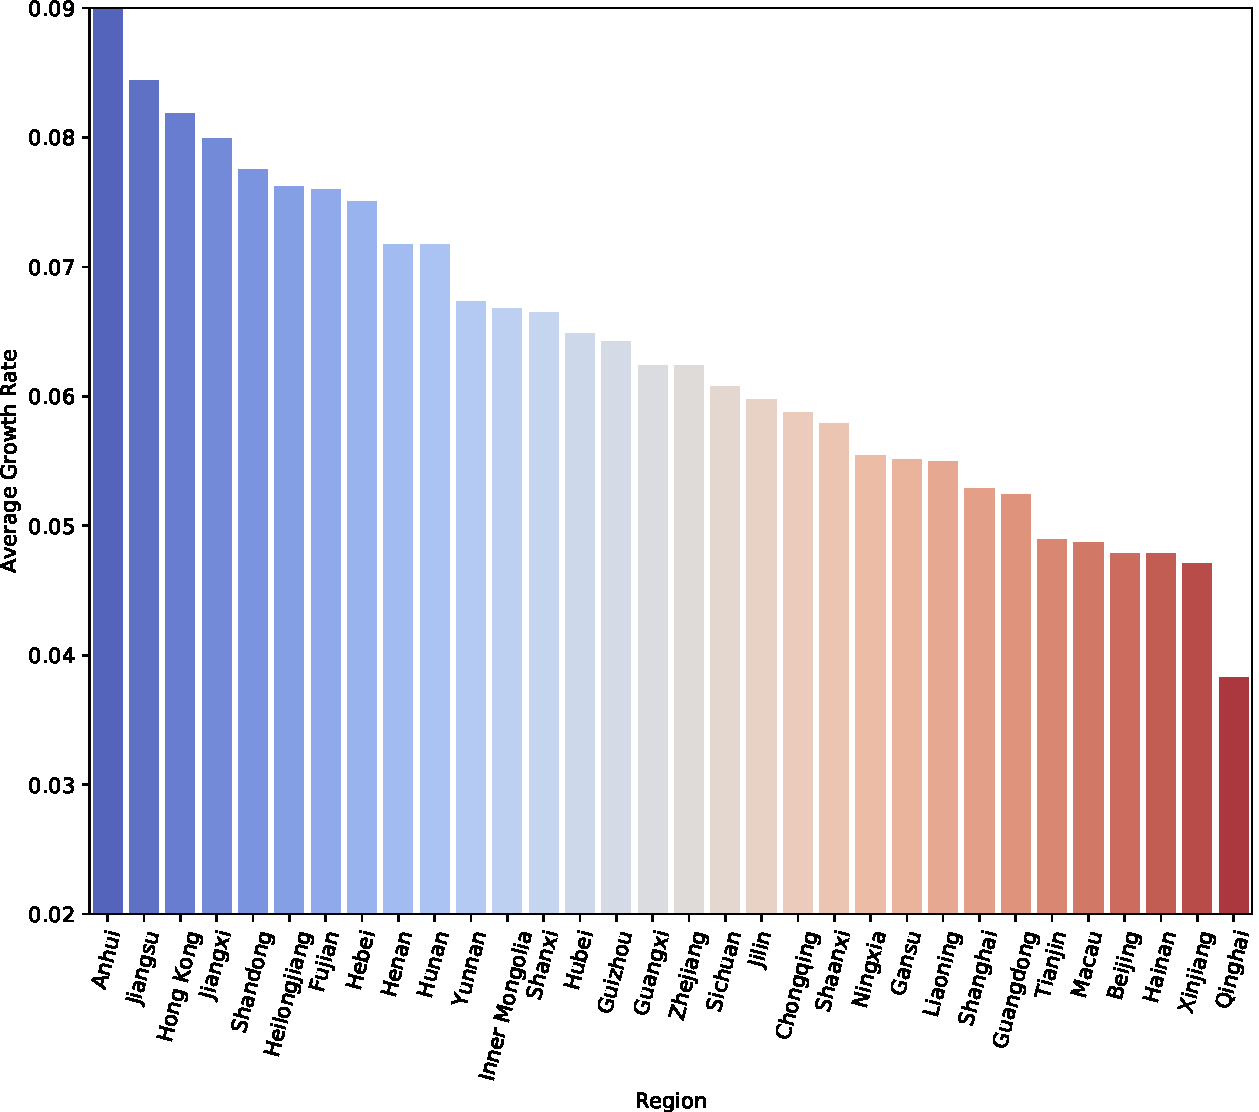
\includegraphics[width=0.8\textwidth]{ly1.pdf}
  \caption{Average Growth Rate of COVID-19 in China}
  \label{fig:ly1}
\end{figure}

Next, we examined the correlation between the average growth rate and the geographical distance to Hubei, the outbreak city of COVID-19. Our conjecture is the average growth rate decreases with an increase in distance. The geographical distance is calculated via the Geopy python library~\cite{geopy}. \cref{fig:ly2} shows the average growth rate by distance to Hubei. The trend matches our expectations. For regions within 1000 km from Hubei, their average growth rate is greater than those distant regions. However, we still observed some counterexamples, for instance, Heilongjiang. Heilongjiang is China's northernmost province which shares a border with Russia, while Hubei is a landlocked province in central China. To figure out possible explanations for Heilongjiang's high average growth rate, we did a literature research for COVID-19 news in Heilongjiang. We found that since early April, there were a large number of imported COID-19 cases from Russia~\cite{heilongjiang}. It is highly possible that these imported cases result in an increase of COVID-19's growth rate.
\begin{figure}[htp]
  \centering
  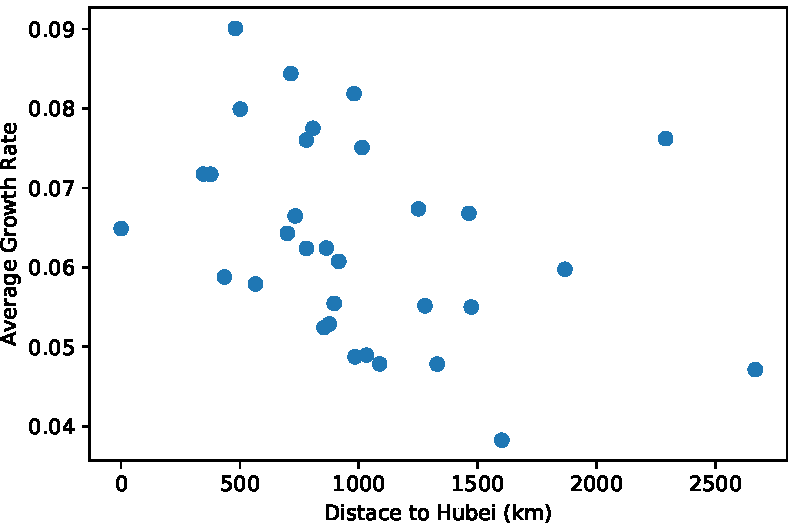
\includegraphics[width=0.6\textwidth]{ly2.pdf}
  \caption{Average Growth Rate by Distance to Hubei}
  \label{fig:ly2}
\end{figure}

Apart from~\cref{fig:ly2}, we also calculated the covariance matrix for the average growth rate and distance (we cannot apply ANOVA here since the average growth rate is not normally distributed). The result is shown in~\cref{eq:3}, where the negative covariance indicates a negative correlation between the two variables.
\begin{equation}
    \bm{cov}(\bm{AverageGrowthRate}, \bm{Distance}) = 
    \begin{bmatrix}
        1.58403777e-04 & -2.48454066e+00 \\
        -2.48454066e+00 & 3.08315655e+05
    \end{bmatrix}\label{eq:3}
\end{equation}

The last analysis we conducted on the COVID-19 Open Research dataset is the ANOVA between the daily growth rates and weather data. We chose four regions for this analysis: Beijing, Guangdong, Liaoning, and Shanghai. These four provinces are located in different areas in China, so that their weather data is distinct. The corresponding mean of the daily growth rate is labeled as $\mu_1$, $\mu_2$, $\mu_3$, and $\mu_4$. For each pair of weather data, a two-way ANOVA is carried out to verify the following hypothesis test:
    \begin{align}
        H_0: & \:\mu_1 = \mu2 = \mu3 = \mu4 \\
        H_1: & \:\mathit{at\:least\:one\:mean\:differs\:from\:others}
    \end{align}

In~\cref{tab:ly3}, we display the result of ANOVA for the mean temperature and total precipitation. It demonstrates that there is no significant difference between growth with distinct mean temperature and total precipitation. For other weather data, the results are similar. Since~\cref{fig:ly2} also illustrates that the average growth rate is between 0.04 - 0.09, which is quite a small range, we can conclude that the weather data has little effect on the spread of COVID-19.

% Please add the following required packages to your document preamble:
% \usepackage{graphicx}
\begin{table}[]
\centering
\caption{ANOVA Result for Mean Temperature and Total Precipitation}
\label{tab:ly3}
\resizebox{0.6\textwidth}{!}{%
\begin{tabular}{lrrrr}
\hline
\multicolumn{1}{c}{\textbf{Measure}} & \multicolumn{1}{c}{\textbf{sum\_sq}} & \multicolumn{1}{c}{\textbf{df}} & \multicolumn{1}{c}{\textbf{F}} & \multicolumn{1}{c}{\textbf{PR(\textgreater{}F)}} \\
\hline
C(temp) & 8.453343e-17 & 2.0 & 7.406908e-16 & 1.000000 \\
C(prcp) & 3.274350e-18 & 2.0 & 2.869020e-17 & 1.000000 \\
C(temp):C(prcp) & 4.702349e-02 & 4.0 & 2.060124e-01 & 0.813969 \\
Residual & 1.352415e+01 & 237.0 & NaN & NaN \\
\hline
\end{tabular}%
}
\end{table}

\subsection{COVID-19 growth interaction with quarantine measures and country}
With the world currently under maintenance and public sentiment deteriorating, it is important to identify
the most efficient quarantine measures so that governments know how to be proactive going forward.
Given a set of countries how do specific quarantine measures affect the growth rate of COVID-19? To analyze this, we used the strictly increasing quantity of total number of tests per capita. Th main external factor which was not taken into account is the fact that the more tests a country performs the more cases typically emerge; i.e., the rate over time
may increase as a result of increased testing and not spread of the disease itself. 
\begin{figure}[h!]
\centering
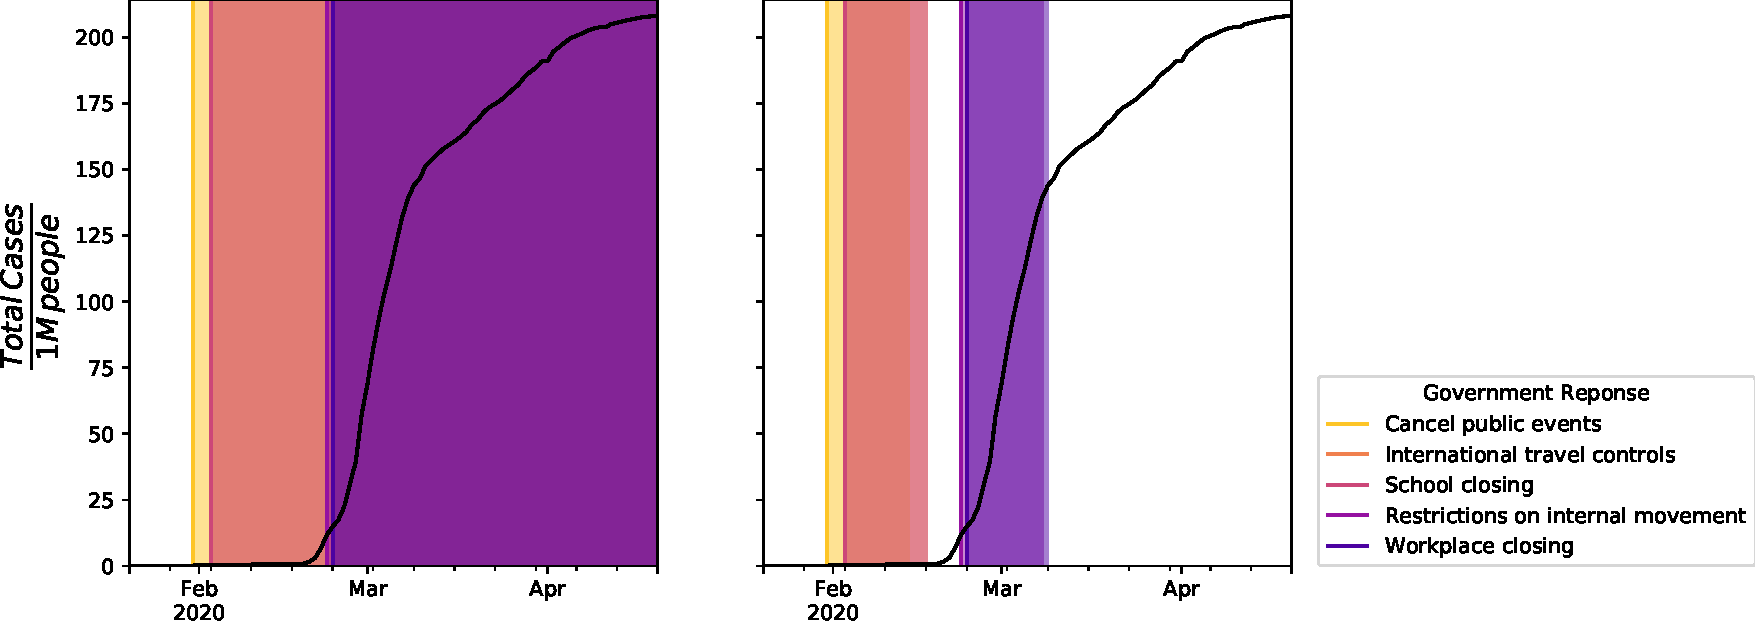
\includegraphics[width=15cm]{mg1.pdf}
\caption{The time series of the total cases per capita for South Korea. (Left) The colored rectangles indicate the active dates for each quarantine measure. (Right) The width is now a 14 day window, approximating the incubation period for COVID-19.}
\label{fig:SKrate}
\end{figure}
Figure \ref{fig:SKrate} demonstrates a time series of total cases for South Korea. The widths
of the colored regions represent different quantities; on the left it demonstrates the total amount
of time certain measures have been in effect while on the right it only shows a 14-day window
after the implementation of each measure. These 14-day windows attempt to account for the time-delayed effect resulting from incubation time. 
The claim that we are pushing is that the rate of change increased until 14 days after the strictest level of quarantine measures were introduced, implying that only then were the measures sufficient.
This behavior is incorporated directly into the analysis. For every quarantine measure, 14 day windows of the time series are taken prior and after each implementation date. The average of the total cases per capita is taken on these windows which results in a triplet of past, present, and future cases per capita values. By assuming exponential growth,
the growth rate before the quarantine measure and after as well as their difference are calculated using
\begin{align}
\rho_{i} &= \frac{1}{\Delta t_{mi}}\log(\frac{\phi_m}{\bar{\phi}_i})\nonumber \\
\rho_{f} &= \frac{1}{\Delta t_{fm}}\log(\frac{\bar{\phi}_{f}}{\phi_m})\nonumber \\
\rho &= \rho_{f}-\rho_{i} \,,
\label{eq:avgrates}
\end{align}
where over-bars denote averages over each window.
By iterating over the countries and government responses, equation (\ref{eq:avgrates}) produces a table of observations on which two-way ANOVA can be applied. Specifically,
the blocks were taken to be the different quarantine measures and the treatments were taken to be the countries. The confidence level is chosen to be 95\% and the corresponding hypothesis set can be written as
\begin{align}
    H_0 &: \mu_0 = \mu_1 = ... = \mu_a \nonumber\\
    H_1 &: \text{any of the means is different} \nonumber
\end{align}
The actual application of ANOVA was straight forward using \texttt{statsmodels} Python API. The results in table \ref{table:mganovaresults} look promising with p-values of 0.037 and 0.000003 for the choice of quarantine measure and country, respectively.

\begin{table}[ht]
\centering
\caption{Two-Way ANOVA results for change in growth rate by factor}
\label{table:mganovaresults}
\begin{tabular}{|c|c|c|c|c|}
\hline
        & Sums of squares & d.o.f. & F-stat & p-value \\ \hline
Type    & 6.757982 & 4 & 2.618791 & 0.037044 \\\hline
Country & 71.847056 & 40 & 1.8343 & 0.000003 \\
\hline
\end{tabular}
\end{table}
\begin{figure}[htb!]
  \centering
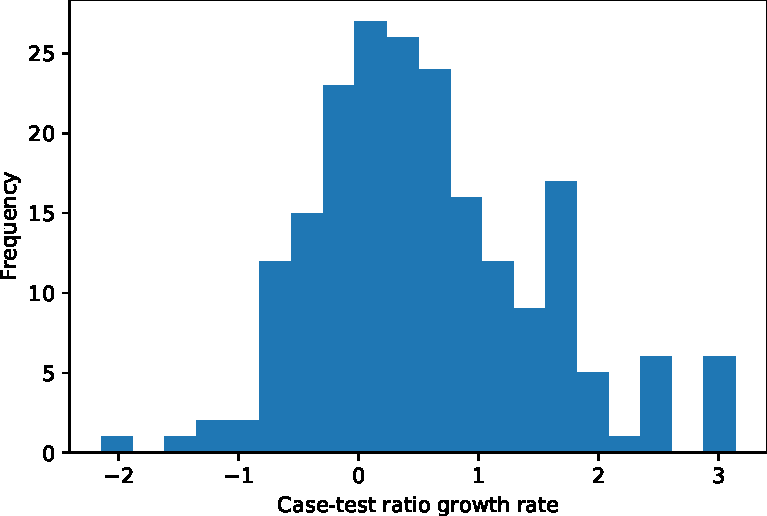
\includegraphics[width=0.4\textwidth]{mg2.pdf}\label{fig:mg2}
  \hfill
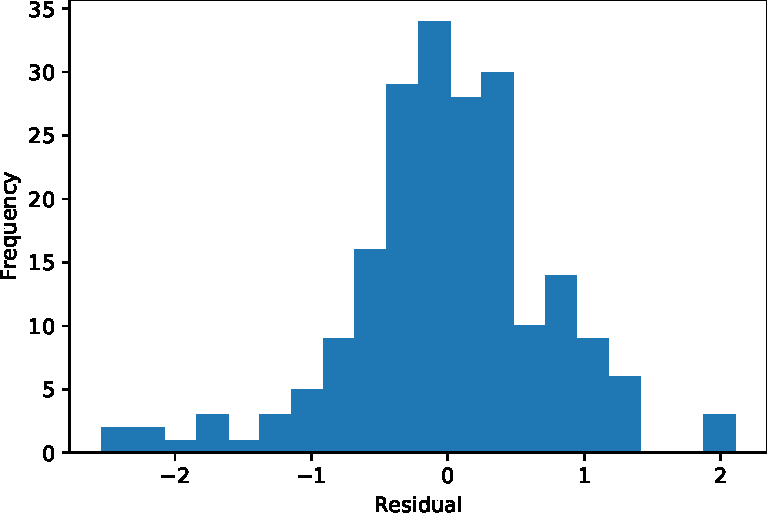
\includegraphics[width=0.4\textwidth]{mg3.pdf}\label{fig:mg3}
  \caption{Observed value and residual distributions}
    \label{TCHist}
\end{figure}
\begin{figure}[htb!]
  \centering
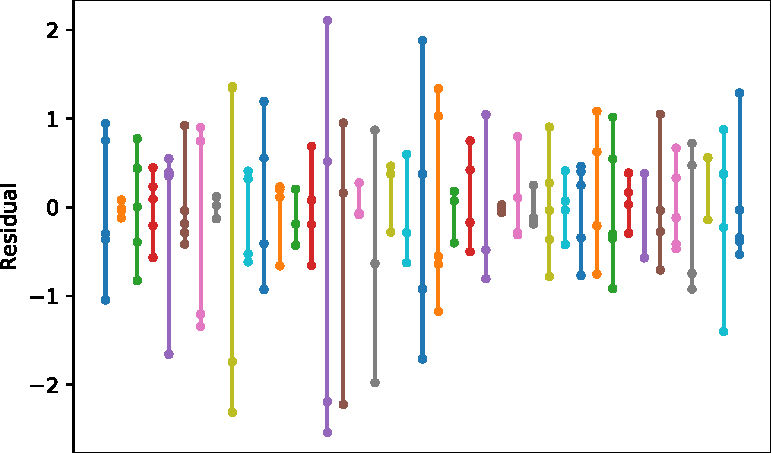
\includegraphics[width=0.4\textwidth]{mg4.pdf}\label{fig:f1}
  \hfill
  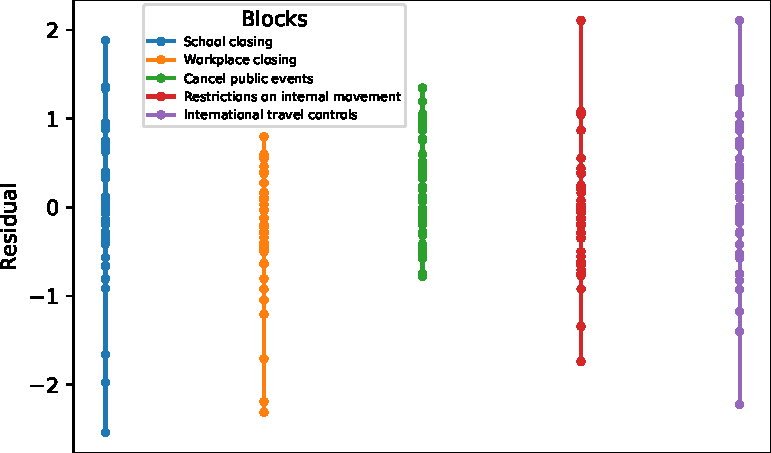
\includegraphics[width=0.4\textwidth]{mg5.pdf}\label{fig:f2}
  \caption{Variance comparisons for treatment residuals (left, countries) and block residuals (right, government responses). There are too many countries to label conveniently but the order from left to right
  is equivalent to the lexicographical ordering in the corresponding
  appendix table.}
    \label{TCvarbar}
\end{figure}
To validate these results the distribution of the observations and their residuals (Figure \ref{TCHist}) as well as variance comparison plots for countries and government responses are displayed (Figure \ref{TCvarbar}). The residuals and observations are approximately normally distributed and the variances for the blocks seem similar. The main area of concern is the variances of each countries' residuals. These disparate variances affect the interpretation of the ANOVA results; especially the effect that the countries have on the rate change. Additionally, these results may be misleading because the quarantine measures overlap with one another; when combined with the time delayed nature of the problem these results should be viewed skeptically. 




\subsection{Doubling Time Analysis}
\begin{table}[htb!]
  \caption{Doubling time of countries}
  \label{table:doubling_countries}
  \begin{adjustbox}{width=\linewidth}
    \csvautotabulartop[respect all]{luke/unfiltered_countries_doubles_0.csv}
    \csvautotabulartop[respect all]{luke/unfiltered_countries_doubles_1.csv}
    \csvautotabulartop[respect all]{luke/unfiltered_countries_doubles_2.csv}
    \csvautotabulartop[respect all]{luke/unfiltered_countries_doubles_3.csv}
  \end{adjustbox}
\end{table}

\if\LukeDoStates1
\begin{table}[htb!]
  \caption{Doubling time of states}
  \label{table:doubling_states}
  \begin{adjustbox}{width=\linewidth}
    \csvautotabulartop[respect all]{luke/unfiltered_states_doubles_0.csv}
    \csvautotabulartop[respect all]{luke/unfiltered_states_doubles_1.csv}
    \csvautotabulartop[respect all]{luke/unfiltered_states_doubles_2.csv}
    \csvautotabulartop[respect all]{luke/unfiltered_states_doubles_3.csv}
  \end{adjustbox}
\end{table}
\fi

To analyse the spread of Covid-19, we looked at the stasticial significance of the doubling time between different countries.
To accomplish this, we used the dataset from John Hopkins, which included cumulative cases for different cities in different regions.
We accumulated the data by region, before remapping the data to consider the number of days since the country first had 100 confirmed cases.
This allows a better inter country comparison.
We then filtered out countries for which had less than 1000 cases, to ensure that enough of the trend could be seen to derive some conclusions from, as well as countries who's reported cases did not increase more than 1\% between the five most recent days (removing \input{luke/unfiltered_countries_removed_growth.csv} due to growth).

\AddLukeFigure{unfiltered}{countries}{Countries}
%Unfiltered Countries
This resulted in \input{luke/unfiltered_countries_remaining_count.csv} countries, of which the minimum time frame was \input{luke/unfiltered_countries_max_timescale.csv}.
To calculate the doubling time for each country, we compared the number of days between the first day of 100 cases and the current day, and the number of doubling between the two dates.
The resulting countries, cumulative cases, and doublings can be seen in Figure \ref{fig:doublings_unfiltered_countries}.

Treating each country as a separate sample, we performed a confidence interval on the expected doubling time, as well as plotting a histogram and box plot, and normality analysis.
We determined that the sample mean was \input{luke/unfiltered_countries_mean.csv}, with a confidence interval \input{luke/unfiltered_countries_ci.csv} with $\alpha=0.05$. 
This is comparable to the results seen in \cite{systemic_review}, where they reference papers with confidence intervals 6.4 to 7.4, and 2.9 to 4.6, where our results fall very close to the first, and larger than \cite{high_contagiousness} where they found a confidence interval for the initial Wuhan outbreak to be 2.3-3.3.
We do note that our data uses much more recent data (up until \input{luke/end_date.csv}), and considers all data reported, where the papers only consider data up to their publication.
Through a normality consideration, we see that we get a p-value of \input{luke/unfiltered_countries_p.csv}, indicating that we can reject the hypothesis that the data is normal with $\alpha=0.05$. 



%\AddLukeFigure{filtered}{countries}{Countries without outliers}
%By repeating the analysis with the two outliers removed (Bahrain, Japan, Denmark), we find a new confidence interval \input{filtered_countries_ci.csv}.
%The new plot can be seen in Figure \ref{fig:test_filtered_countries}, where a normality p-value of \input{filtered_countries_p.csv}, indicating that the data does in fact follow a normal distribution.


\if\LukeDoStates1
\AddLukeFigure{unfiltered}{states}{States}
We also looked at the distribution of doubling within the United States on a per state basis. The same initial filtering was done, which removed \input{luke/unfiltered_states_removed_end.csv} due to not having more than 1000 cases.
The new plot can be seen in Figure \ref{fig:test_unfiltered_states}, where a normality p-value of \input{luke/unfiltered_countries_p.csv}, indicating that the data does in fact follow a normal distribution.
\fi


\subsection{Basic Reproduction Number Analysis}
A meta-analysis was performed using published estimates for COVID-19's $R_0$. From the sample captured by the $R_0$ data set provided in Appendix A, descriptive statistics were used to quantify and visualize the central tendency and spread of these estimates. Table \ref{tab:table1} summarizes some of the relevant numeric properties of the sample. Note that a mean $R_0$ of 3.45 is interpreted as an infected person transmitting the virus to 3.45 others, on average.

\begin{table}[htp]
  \begin{center}
    \caption{Descriptive Statistics for the $R_0$ Estimates.}
    \label{tab:table1}
    \begin{tabular}{l|r}
    \hline \hline
      \textbf{Measure} & \textbf{Result} \\
      \hline
      Mean & 3.45\\
      Median (Q2) & 3.01\\
      Minimum & 1.90\\
      Maximum & 6.49\\
      Range & 4.59\\
      Standard Deviation & 1.41\\
      Variance & 1.99\\
      1\textsuperscript{st} Quartile (Q1) & 2.27\\
      3\textsuperscript{rd} Quartile (Q3) & 4.43\\
      Interquartile Range (IQR) & 2.16\\
      \hline \hline
    \end{tabular}
  \end{center}
\end{table}

Using the quartile results in Table \ref{tab:table1}, a box plot of the $R_0$ estimates was plotted in figure \ref{R0DescStats} (a). To check for outliers, the lower bound and upper bound were calculated to be -0.96 and 7.66, respectively. Because all of the $R_0$ estimates used in the current analysis are contained within the range between the lower and upper bounds, none of the estimates in the data set were found to be outliers. To further visualize the spread of data, a scatter plot is provided in figure \ref{R0DescStats} (b). The magnitude of $R_0$ is plotted against the width of each estimate's 95\% confidence interval, which was calculated by taking the difference between the confidence interval's upper and lower bounds.

\begin{figure}[!tbp]
  \centering
  \subfloat[$R_0$ Box Plot]{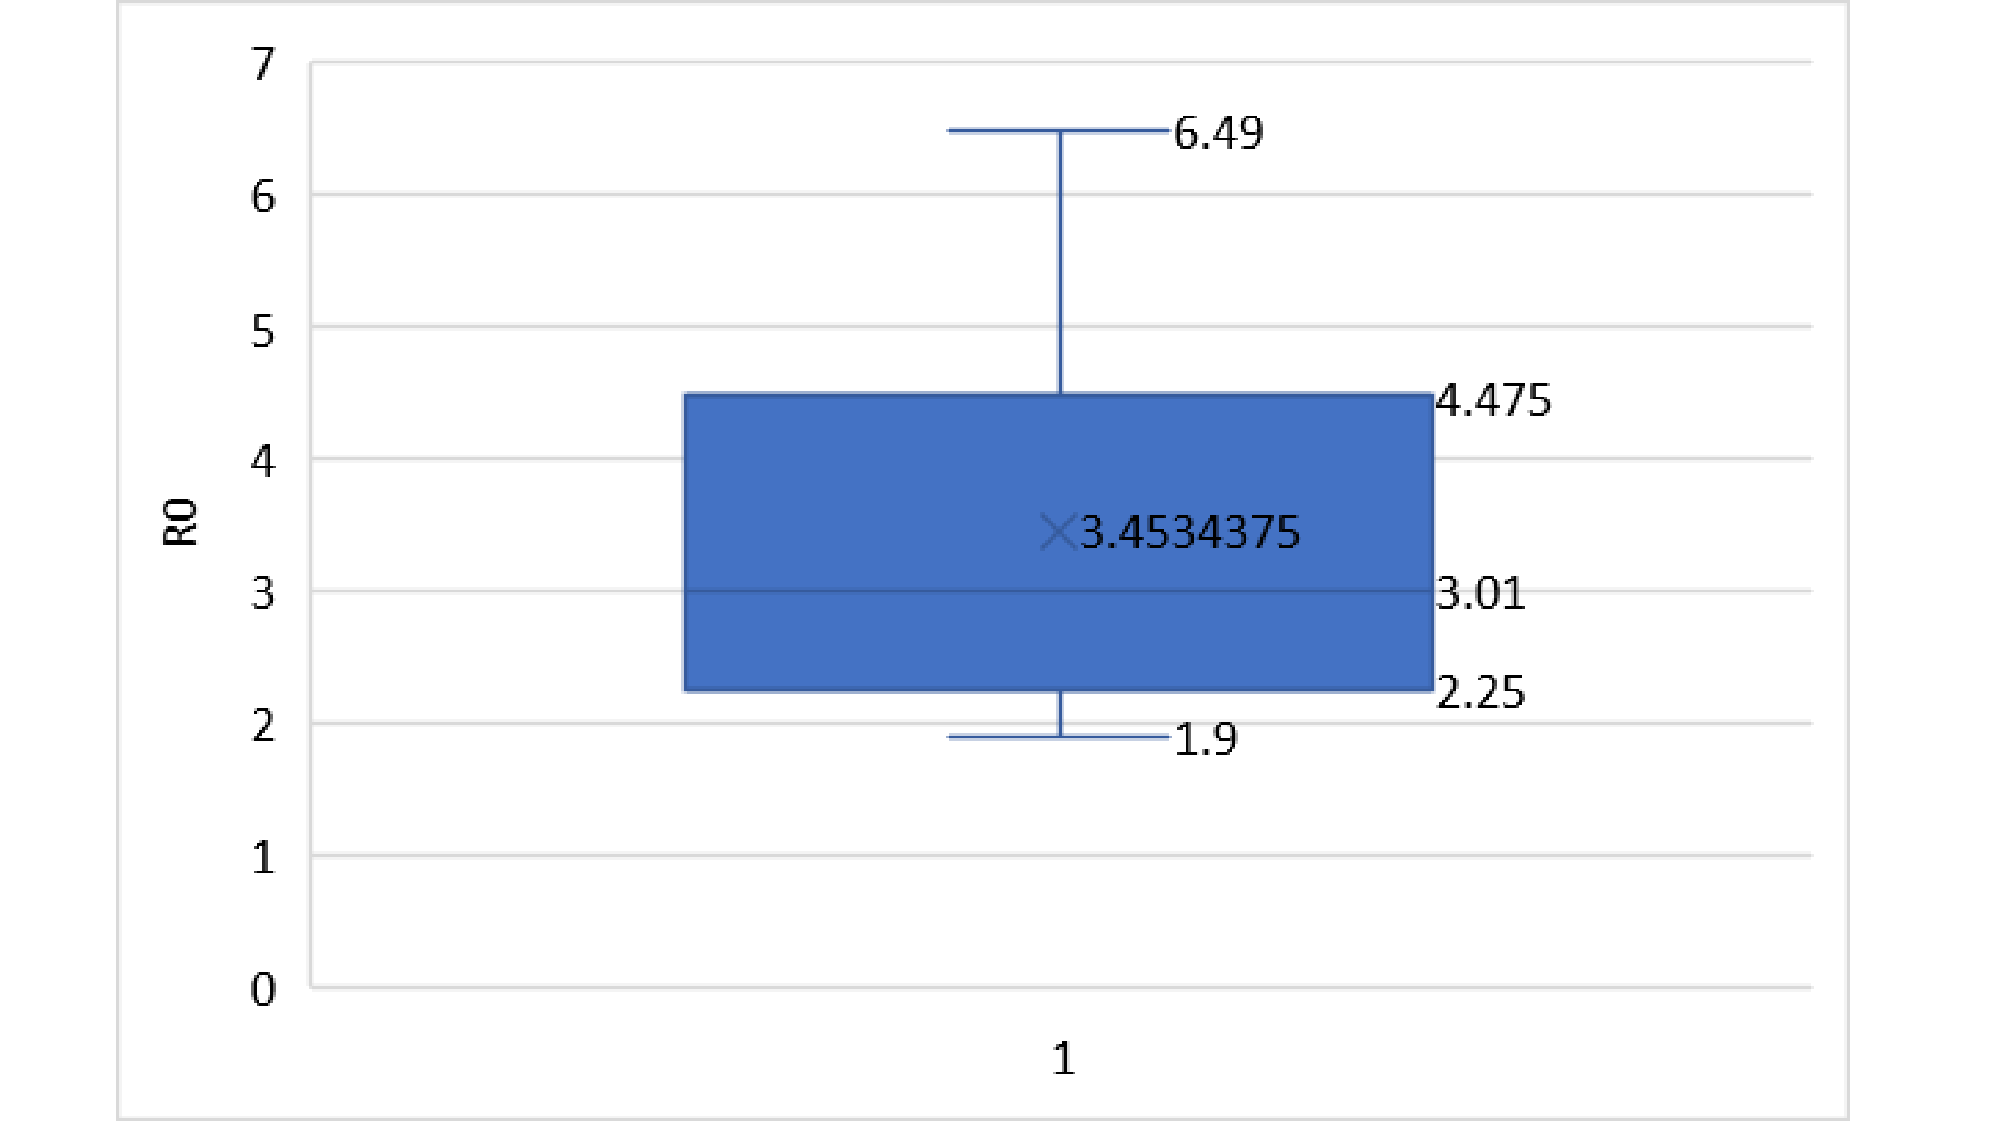
\includegraphics[width=0.5\textwidth]{sm1.pdf}\label{fig:f1}}
  \hfill
  \subfloat[$R_0$ Scatter Plot]{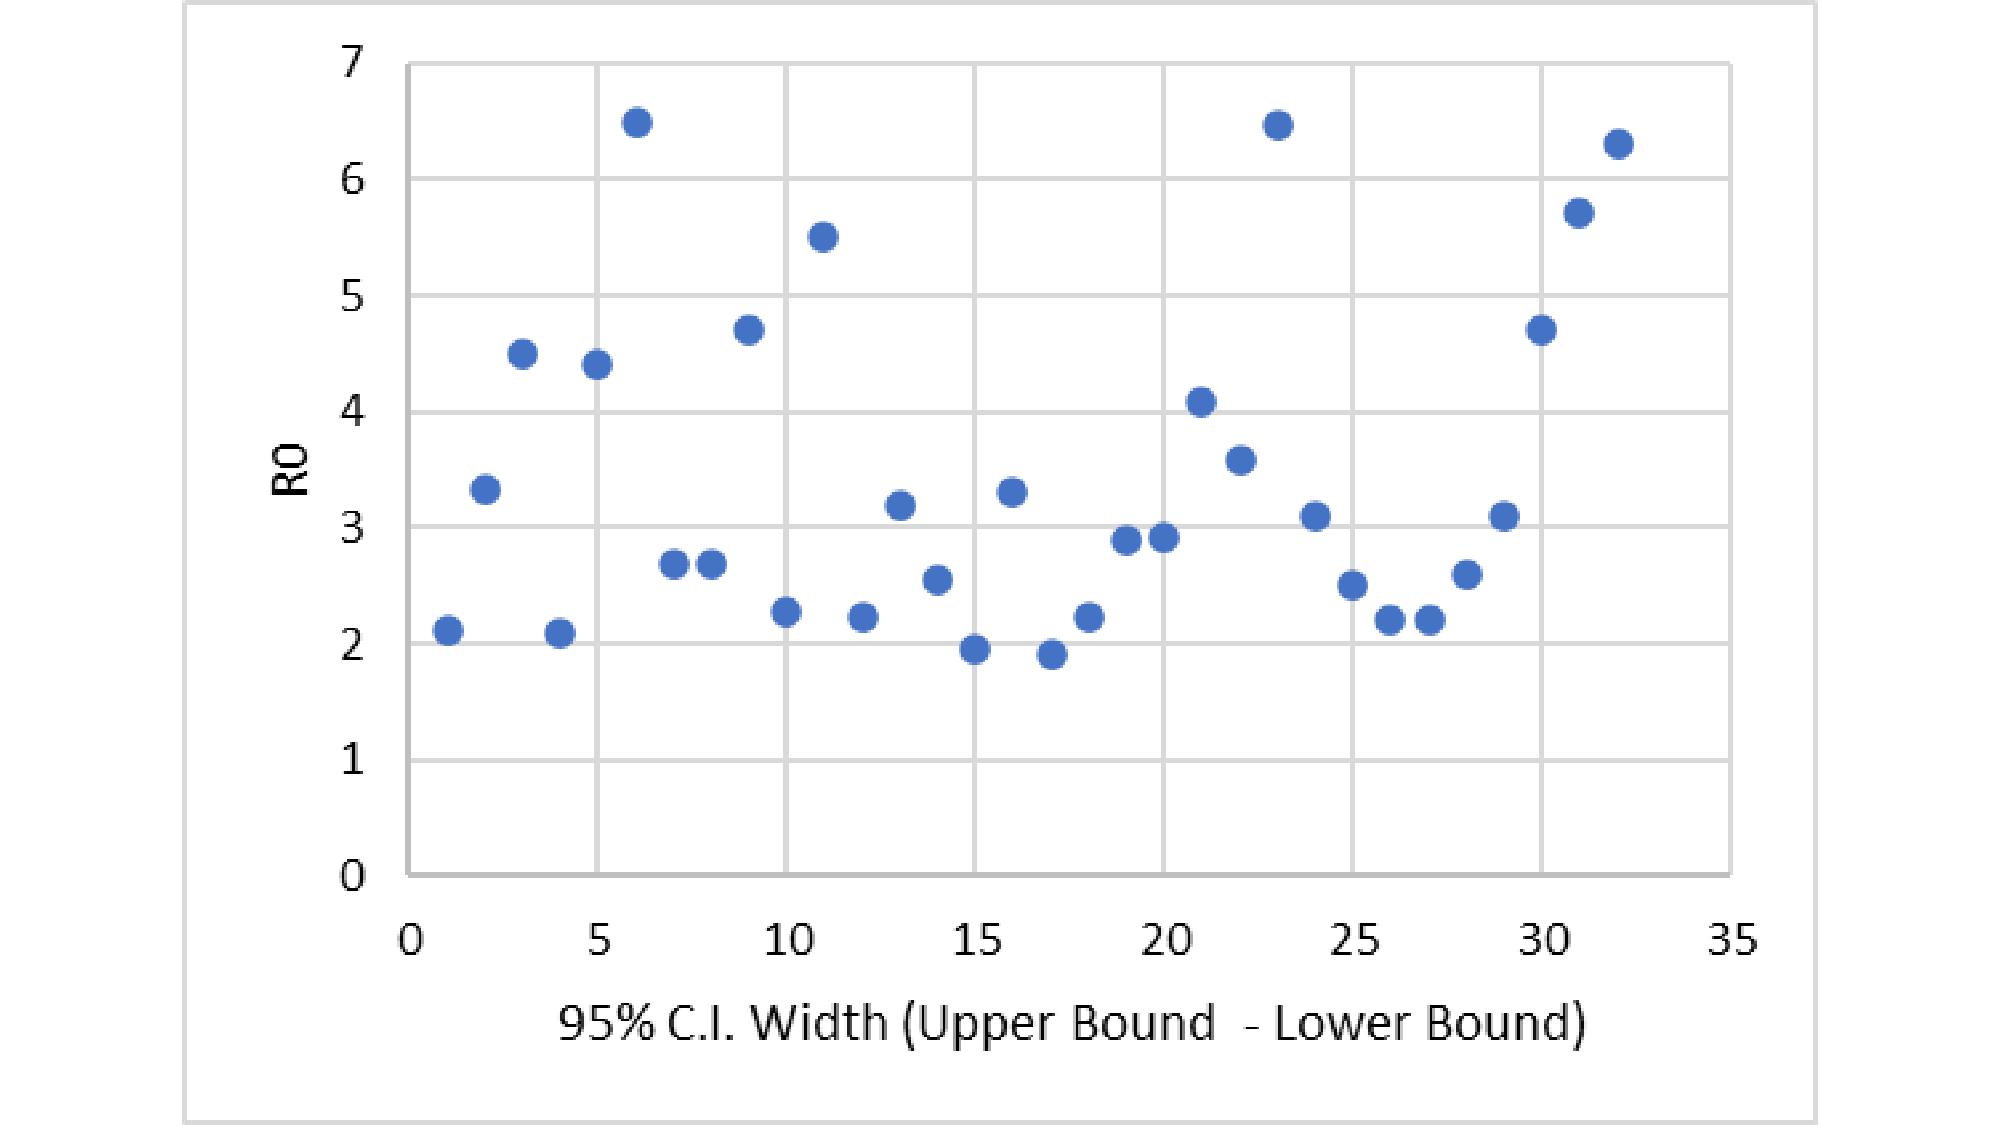
\includegraphics[width=0.5\textwidth]{sm2.pdf}\label{fig:f2}}
  \caption{Descriptive Statistics for $R_0$ Estimates.}
    \label{R0DescStats}
\end{figure}

Next, we aim to investigate the relationship between the magnitude of the $R_0$ estimate and the study date. The goal of this analysis is to indicate whether the transmission of the virus has grown or lessened over time. A Chinese governmental ban on public transportation that was invoked on January 23, 2020 for five major cities (Wuhan, Huanggang, Ezhou, Chibi and Zhijiang) \cite{2}. Thus, we choose to divide the data set into two groups: set 1 includes $R_0$ estimates from studies that used COVID-19 case data leading up to and including January 23, 2020 and set 2 data includes $R_0$ estimates from studies that considered reported cases of COVID-19 since January 23, 2020. The sample size of set 1 and set 2 are equal with 16 estimates in each category. Histograms to show the distribution of both data sets are provided in figure \ref{R0Hists}. Both distributions are positively skewed, favoring lower magnitude $R_0$ estimates.

\begin{figure}[!tbp]
  \centering
  \subfloat[$R_0$ Data Set 1 Histogram]{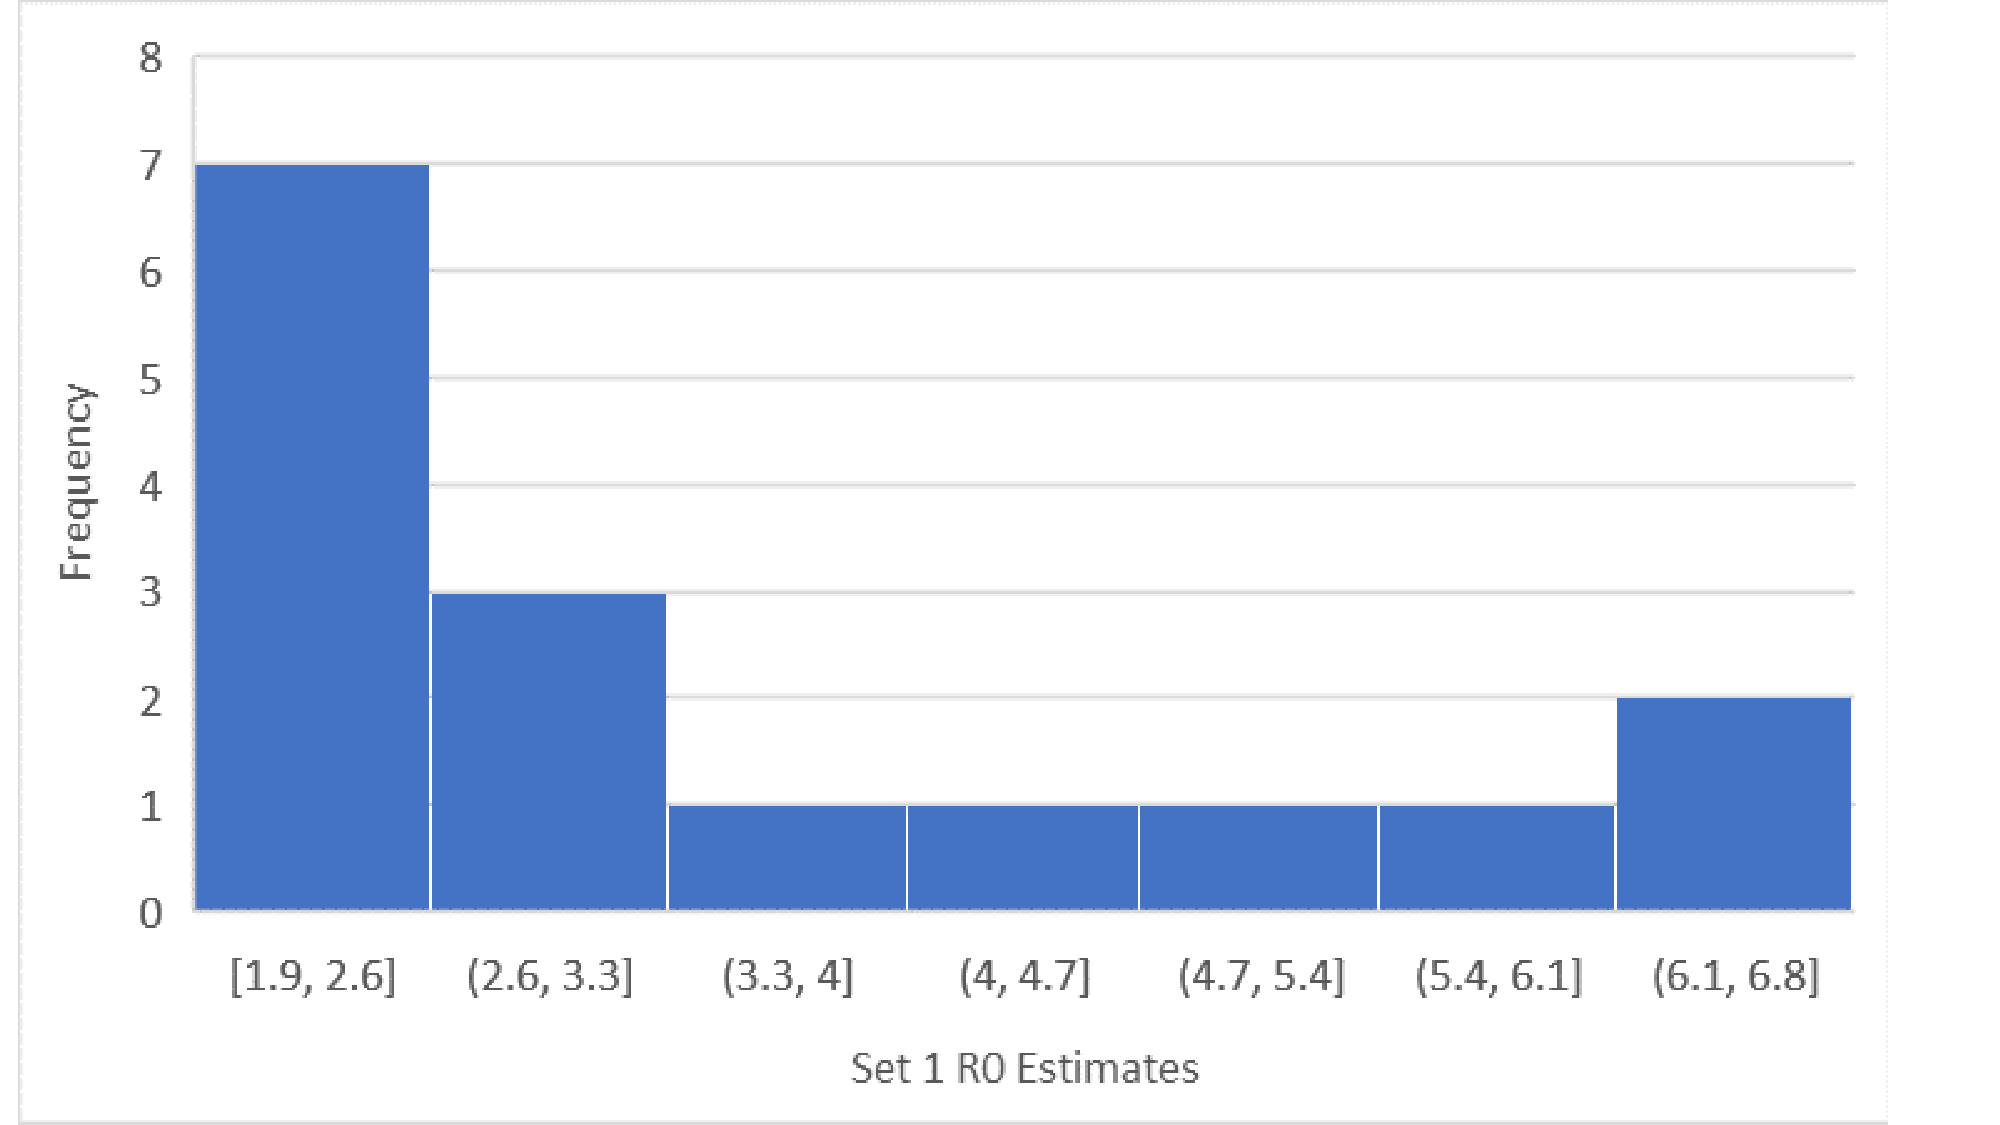
\includegraphics[width=0.5\textwidth]{sm6.pdf}\label{fig:f1}}
  \hfill
  \subfloat[$R_0$ Data Set 2 Histogram]{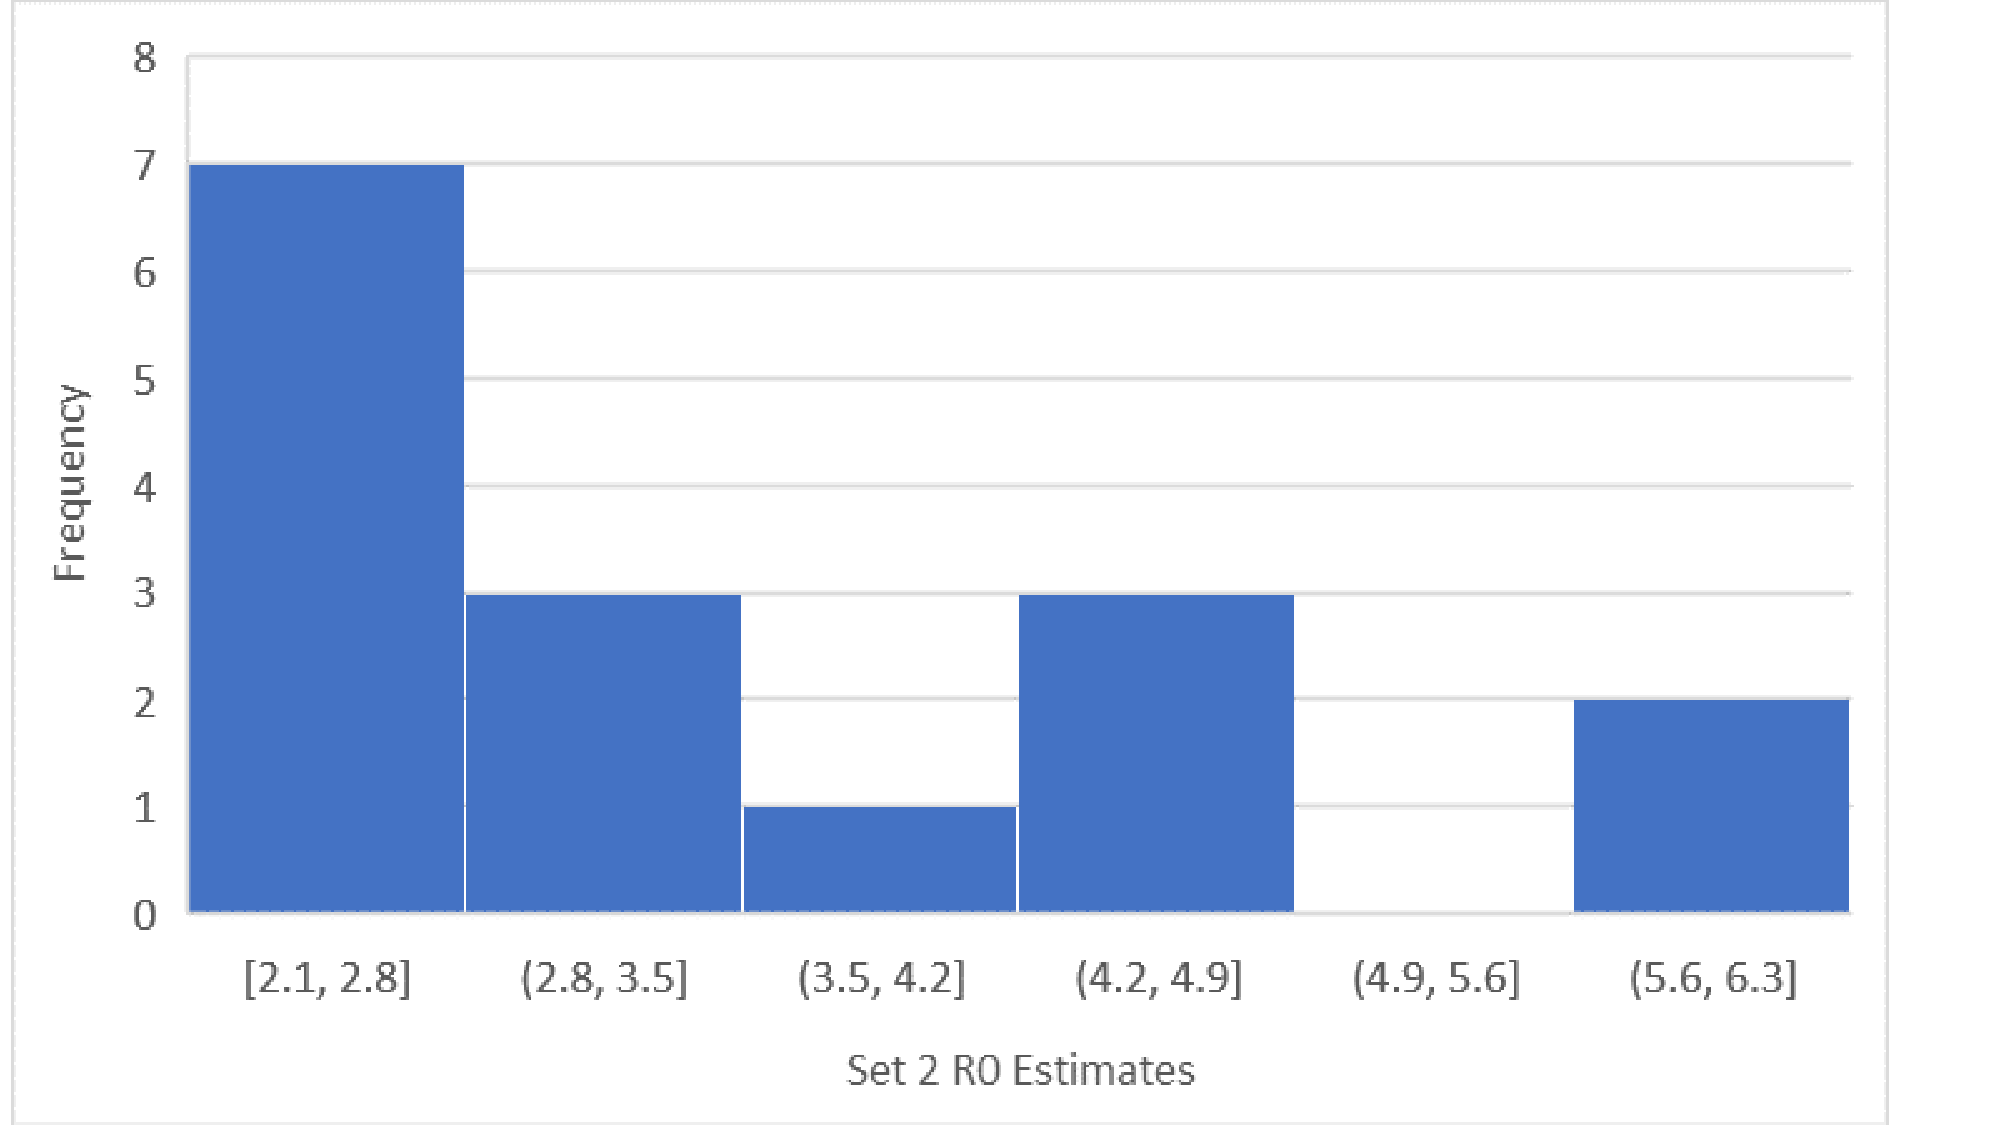
\includegraphics[width=0.5\textwidth]{sm7.pdf}\label{fig:f2}}
  \caption{Distributions of Set 1 and Set 2 Data for $R_0$ Estimates}
    \label{R0Hists}
\end{figure}

A simple linear regression analysis is performed using the study date as the independent/predictor variable and the $R_0$ estimate as the dependent/response variable. To turn the study date into an integer, the earliest study date was given a value of zero and each day thereafter is incremented by a value of one. The resulting regression equation is \^{y} = 0.00158X + 3.4152. Because the slope of the regression line is nearly zero, we conclude that there is very little correlation between the study date and R0 estimate. The linear regression results are plotted in figure \ref{R0Reg}. A summary of the regression results is provided in table \ref{tab:table2}.

\begin{figure}[h!]
  \centering
  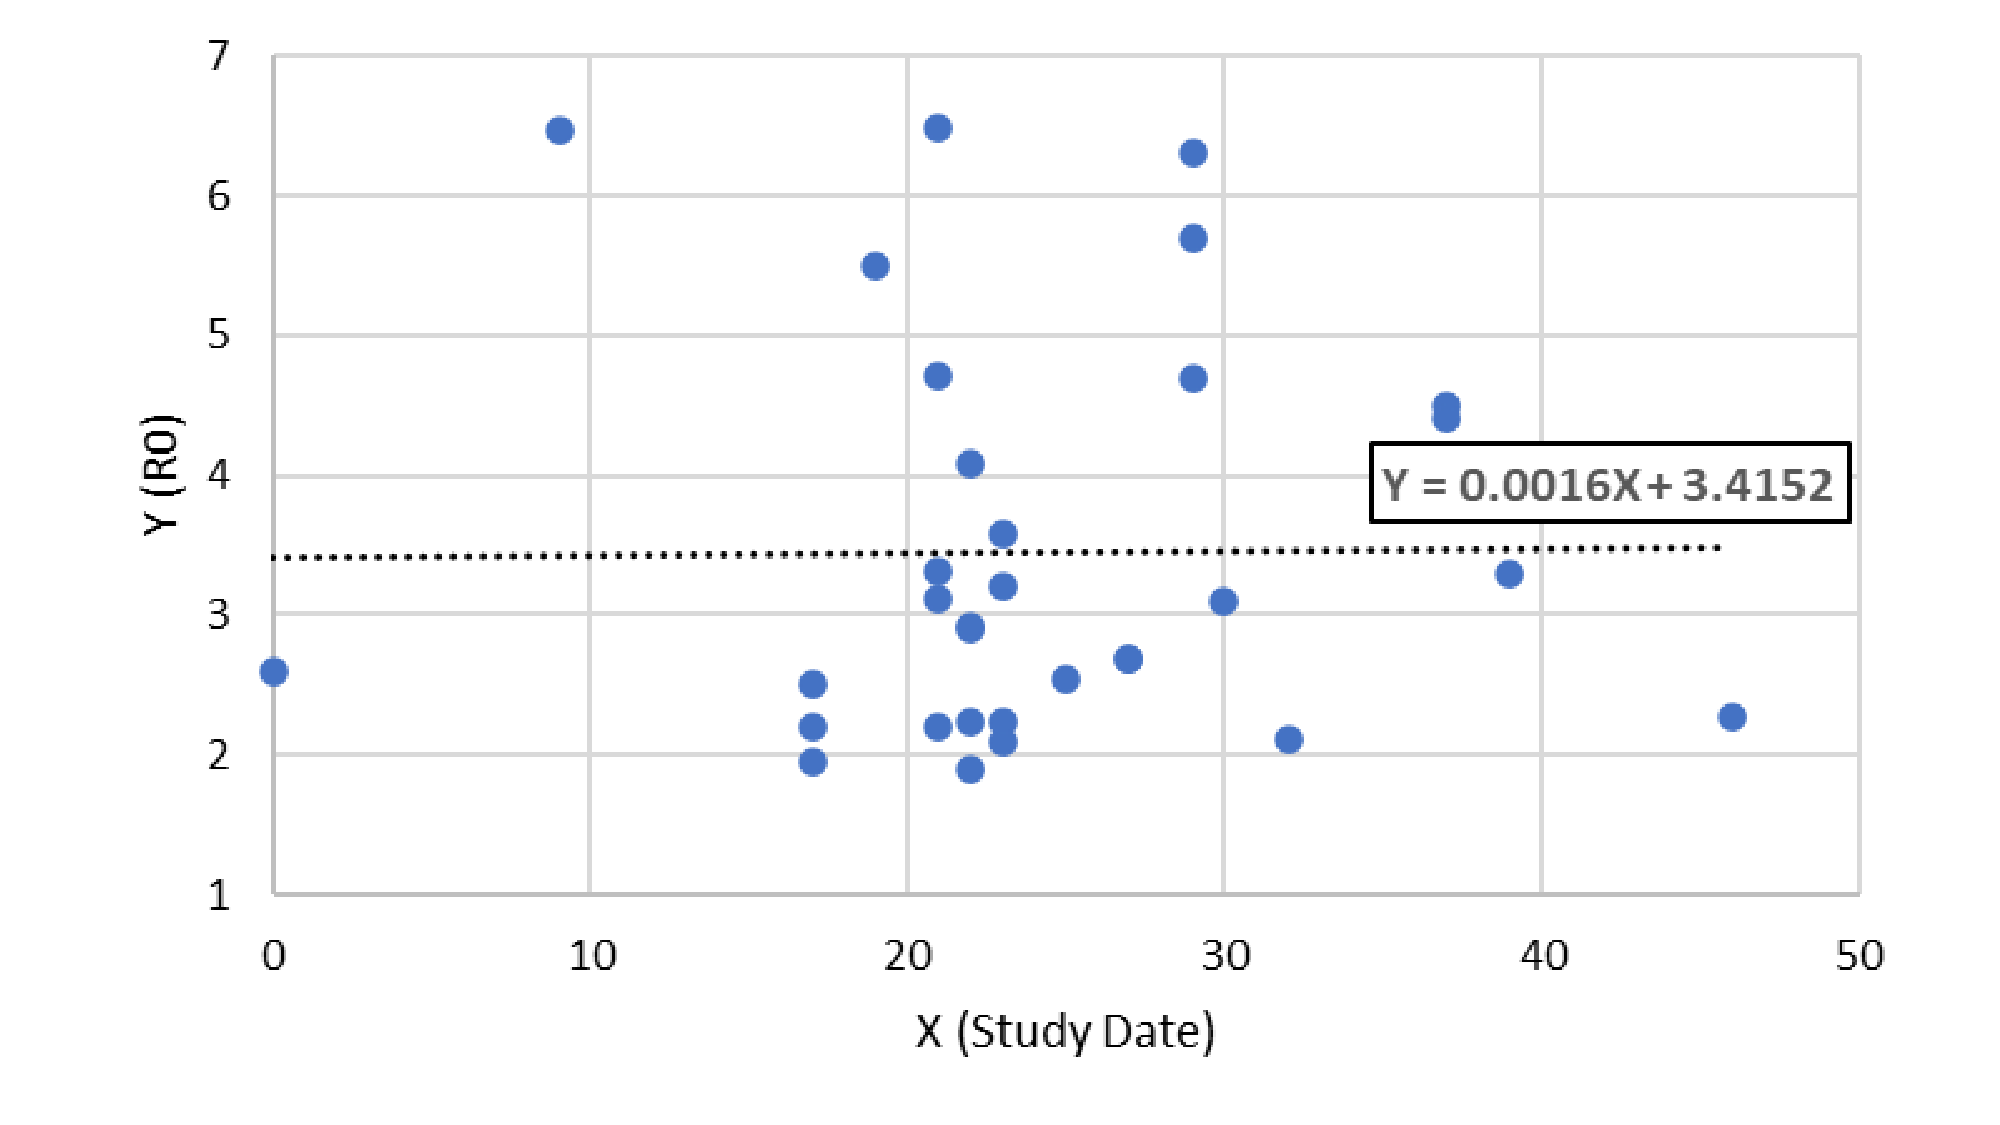
\includegraphics[width=10cm]{sm5.pdf}
  \caption{Linear Regression Results for $R_0$ Estimates}
  \label{R0Reg}
\end{figure}

\begin{table}[h!]
  \begin{center}
    \caption{Simple Linear Regression Results for $R_0$ Estimates.}
    \label{tab:table2}
    \begin{tabular}{l|r}
    \hline \hline
      \textbf{Regression Result} & \textbf{Value} \\
      \hline
      $\bar{X}$ & 24.16\\
      $\bar{Y}$ & 3.45\\
      $\hat{\beta_{0}}$ & 3.415\\
      $\hat{\beta_{1}}$ & 0.0016\\
      $SS_{Error}$ & 61.5468\\
      $SS_{Total}$ & 61.5525\\
      $SS_{Regression}$ & 0.0057\\
      Means Squared Error (MSE) & 2.0516\\
      $\alpha$ & 0.05\\
      df (n - 2) & 30\\
      $t_{\alpha/2, n-2}$ & 2.042\\
      Margin of Error of C.I. (E) & 0.5337\\
      95\% C.I. for \^{y} = 3.45 & (2.9163, 3.9837)\\
      \hline \hline
    \end{tabular}
  \end{center}
\end{table}

\section{Implications}
Looking at the distribution of doubling time for various countries, a number of implications arise.
First, a number of countries considered to be first world have short doubling time - notable US, the UK, Spain, Canada, France and Germany.
This could be related to the amount of testing done, as well as how quickly the country responded as a whole.
Secondly, as the doubling time does appear to follow a normal distribution, more advance analysis techniques could be used which require a normal distribution.


The initial hypothesis that $R_0$ would decrease over time in response to social distancing and restrictions on public gatherings was not confirmed in the current analysis. Instead, no significant correlation between study dates and estimated $R_0$ was found. Nonetheless, we do not conclude that these variables are entirely unrelated. Instead, it is proposed that more time and more observations are necessary to observe a relationship between these variables using simple linear regression.
%Short individual implications
The implications of the two-way ANOVA analysis with countries and
government quarantine responses are that both the
factors have statistically significant effects. If the results
are taken seriously then this would imply that a custom tailored approach should be considered when decided upon the quarantine measures to enact.
%Then combination of those
\section{Future Work}
%Lechen's Stuff
The analysis on the effect of geography data indicates that it has a negative correlation with COVID-19's spread. We plan to further analyze this relationship in a fine-grained manner (e.g., analyzing the growth rate for each city in China). In addition, we will also examine other weather data to find potential factors that affect the spread of COVID-19.

%Matt's Stuff
The analysis on the effect of different quarantine measures do not take a number of details into account. The most important of which is the fact that the quarantine measures are not independent as they are overlap in regards to time. Therefore, to analyze quarantine
measures correctly there should likely be a different method developed which accounts for this. Other considerations also need to be made such as how the number of cases depends on the number of tests.

%Luke's Stuff
Given the doubling rate per country, it would be possible to attempt to correlate factors of countries, such as population density, to see what factors impact the doubling time. 
Furthermore, one could look into how the doubling time changes with respect to the measures put in place as a proxy for determining the effectiveness of the measures.

%Sara's Stuff
Given more time, extending the literature review for published estimates of $R_0$ for COVID-19 in China to produce a greater sample size would strengthen the statistical analyses performed for the current meta-analysis. If enough observations were collected in each data set such that n > 30 for estimates using reported cases prior to (data set 1) and after (data set 2) January 23, 2020, then using the assumption of approximately normally-distributed data could expand the number of inferences that could be drawn on this data.

\begin{thebibliography}{}
\bibitem{1} 
World Health Organization. Coronavirus disease 2019 (COVID-19) situation reports, 2020.
\bibitem{2} 
BBC NEWS. "Coronavirus: Wuhan Shuts Public Transport over Outbreak." Jan. 23, 2020.
\bibitem{john_hopkins}
Johns Hopkins University Center for Systems Science and Engineering (JHU CSSE)
\bibitem{owid}
Our World in Data. Joe Hasell, Esteban Ortiz-Ospina, Edouard Mathieu, Hannah Ritchie, Diana Beltekian and Max Roser \url{https://github.com/owid/covid-19-data/tree/master/public/data/}
\bibitem{find}
Foundation for Innovative New Diagnostics. COVID-19 Testing Tracker. 
\url{https://finddx.shinyapps.io/FIND\_Cov\_19\_Tracker/}
\bibitem{govtresponse}
A. Petherick, T. Hale, T. Phillips, S. Webster, Variation in Government Responses to COVID-19. Preprint
\url{https://www.bsg.ox.ac.uk/research/publications/variation-government-responses-covid-19}
\bibitem{systemic_review}
  M. Park, A. R. Cook, J. T. Lim, Y. Sun, and B. L. Dickens, “A Systematic Review of COVID-19 Epidemiology Based on Current Evidence,” Journal of Clinical Medicine, vol. 9, no. 4, p. 967, Apr. 2020, doi: 10.3390/jcm9040967.
\bibitem{high_contagiousness}
  S. Sanche, Y. T. Lin, C. Xu, E. Romero-Severson, N. Hengartner, and R. Ke, “Early Release - High Contagiousness and Rapid Spread of Severe Acute Respiratory Syndrome Coronavirus 2 - Volume 26, Number 7—July 2020 - Emerging Infectious Diseases journal - CDC,” doi: 10.3201/eid2607.200282.
\bibitem{Lai}
Lai A, Bergna A, Acciarri C, Galli M, Zehender G. Early Phylogenetic Estimate of the Effective Reproduction Number Of Sars‐CoV‐2. Journal of Medical Virology. 2020.
\bibitem{Biao}
Tang B, Wang X, Li Q, Bragazzi NL, Tang S, Xiao Y, et al. Estimation of the transmission risk of the 2019-nCoV and its implication for public health interventions. Journal of Clinical Medicine. 2020;9(2):462.
\bibitem{WHO}
Liu Y, Gayle AA, Wilder-Smith A, Rocklöv J. The reproductive number of COVID-19 is higher compared to SARS coronavirus. Journal of Travel Medicine. 2020.
\bibitem{Imai}
Imai N, Cori A, Dorigatti I, Baguelin M, Donnelly CA, Riley S, et al. Report 3: transmissibility of 2019-nCov. Reference Source. 2020.
\bibitem{Riou}
Riou J, Althaus CL. Pattern of early human-to-human transmission of Wuhan 2019-nCoV. bioRxiv. 2020.
\bibitem{Zhou}
Zhou C. Evaluating new evidence in the early dynamics of the novel coronavirus COVID-19 outbreak in Wuhan, China with real time domestic traffic and potential asymptomatic transmissions. medRxiv. 2020.
\bibitem{Shao}
Shao N, Cheng J, Chen W. The reproductive number R0 of COVID-19 based on estimate of a statistical time delay dynamical system. medRxiv. 2020.
\bibitem{Shen}
Shen M, Peng Z, Xiao Y, Zhang L. Modelling the epidemic trend of the 2019 novel coronavirus outbreak in China. bioRxiv. 2020.
\bibitem{Read}
Read JM, Bridgen JR, Cummings DA, Ho A, Jewell CP. Novel coronavirus 2019-nCoV: early estimation of epidemiological parameters and epidemic predictions. medRxiv. 2020.
\bibitem{Li}
Li Q, Guan X, Wu P, Wang X, Zhou L, Tong Y, et al. Early transmission dynamics in Wuhan, China, of novel coronavirus–infected pneumonia. New England Journal of Medicine. 2020.
\bibitem{Du}
Du Z, Wang L, Cauchemez S, Xu X, Wang X, Cowling BJ, et al. Risk for Transportation of 2019 Novel Coronavirus (COVID-19) from Wuhan to Cities in China. medRxiv. 2020.
\bibitem{Li2}
Li R, Pei S, Chen B, Song Y, Zhang T, Yang W, et al. Substantial undocumented infection facilitates the rapid dissemination of novel coronavirus (COVID-19). medRxiv. 2020.
\bibitem{Liu}
Liu T, Hu J, Kang M. Transmission dynamics of 2019 novel coronavirus (2019-nCoV). bioRxiv 2020; published online Jan 26. DOI.10(2020.01):25.919787.
\bibitem{Liu2}
Liu Y, Gayle AA, Wilder-Smith A, Rocklöv J. The reproductive number of COVID-19 is higher compared to SARS coronavirus. Journal of Travel Medicine. 2020.
\bibitem{Cao}
Cao Z Zhang Q, Lu X et al. Estimating the effective reproduction number of the 2019-nCoV in China. medRxiv 2020.
\bibitem{Jung}
Jung S-m, Akhmetzhanov AR, Hayashi K, Linton NM, Yang Y, Yuan B, et al. Real-Time Estimation of the Risk of Death from Novel Coronavirus (COVID-19) Infection: Inference Using Exported Cases. Journal of Clinical Medicine. 2020;9(2):523.
\bibitem{Zhao}
Zhao S, Lin Q, Ran J, Musa SS, Yang G, Wang W, et al. Preliminary estimation of the basic reproduction number of novel coronavirus (2019-nCoV) in China, from 2019 to 2020: A data-driven analysis in the early phase of the outbreak. International Journal of Infectious Diseases. 2020.
\bibitem{Zhou2}
Zhang KK, Xie L, Lawless L, Zhou H, Gao G, Xue C. Characterizing the transmission and identifying the control strategy for COVID-19 through epidemiological modeling. medRxiv. 2020.
\bibitem{Majumder}
Majumder MS, Rivers C, Lofgren E, Fisman D. Estimation of MERS-coronavirus reproductive number and case fatality rate for the spring 2014 Saudi Arabia outbreak: insights from publicly available data. PLoS Currents. 2014;6.
\bibitem{Joseph}
Wu JT, Leung K, Leung GM. Nowcasting and forecasting the potential domestic and international spread of the 2019-nCoV outbreak originating in Wuhan, China: a modelling study. The Lancet. 2020.
\bibitem{Sanche}
Sanche S, Lin YT, Xu C, Romero-Severson E, Hengartner NW, Ke R. The Novel Coronavirus, 2019-nCoV, is Highly Contagious and More Infectious Than Initially Estimated. arXiv preprint arXiv:200203268. 2020.
\bibitem{Park}
Park SW, Champredon D, Earn DJ, Li M, Weitz JS, Grenfell BT, et al. Reconciling early-outbreak preliminary estimates of the basic reproductive number and its uncertainty: a new framework and applications to the novel coronavirus (2019-nCoV) outbreak. medRxiv. 2020.
\bibitem{Muniz}
Muniz-Rodriguez K, Chowell G, Cheung C-H, Jia D, Lai P-Y, Lee Y, et al. Epidemic doubling time of the COVID-19 epidemic by Chinese province. medRxiv. 2020.
\bibitem{Zhang}
Zhang S, Diao M, Yu W, Pei L, Lin Z, Chen D. Estimation of the reproductive number of Novel Coronavirus (COVID-19) and the probable outbreak size on the Diamond
Princess cruise ship: A data-driven analysis. International Journal of Infectious Diseases. 2020]
\bibitem{covid19weather}
Davide Bonin. Weather Data for COVID-19 Data Analysis, 2020.
\url{https://www.kaggle.com/davidbnn92/weather-data-for-covid19-data-analysis}
\bibitem{weatherdata}
NOAA. Global Surface Summary of the Day, 2020.
\url{https://www.kaggle.com/noaa/gsod}
\bibitem{normaltest}
Wikipedia. D'Agostino's K-squared test, 2019.
\url{https://en.wikipedia.org/wiki/D\%27Agostino%27s_K-squared_test}
\bibitem{geopy}
Geopy. Geopy Documentation, 2020.
\url{https://geopy.readthedocs.io/en/stable/}
\bibitem{heilongjiang}
ABC News. China moves to block new virus flare-up on Russian border, 2020.
\url{https://abcnews.go.com/International/wireStory/china-moves-block-virus-flare-russian-border-70134699}
\end{thebibliography}

\pagebreak
\appendixpage
\appendix
\section{Basic Reproduction Number Data Set}

\begin{center}
\begin{tabular}{|c|c|c|c|c|} 
\hline
Study & $R_0$ & 95\% CI Lower Bound & 95\% CI Upper Bound & Study Date\\ \hline
Lai et al. \cite{Lai} & 2.60 & 2.10 & 5.10 & 01/01/2020 \\ \hline
Biao \cite{Biao} & 6.47 & 5.71 & 7.23 & 01/10/2020 \\ \hline
WHO \cite{WHO} & 1.95 & 1.40 & 2.50 & 01/18/2020 \\ \hline
Imai \cite{Imai} & 2.50 & 1.50 & 3.50 & 01/18/2020 \\ \hline
Riou \& Althaus \cite{Riou} & 2.20 & 1.40 & 3.80 & 01/18/2020 \\ \hline
Zhou et al. \cite{Zhou2} & 5.50 & 5.30 & 5.80 & 01/20/2020 \\ \hline
Shao et al. \cite{Shao} & 3.32 & 3.25 & 3.4 & 01/22/2020 \\ \hline
Shen et al. \cite{Shen} & 6.49 & 6.31 & 6.66 & 01/22/2020 \\ \hline
Shen et al. \cite{Shen} & 4.71 & 4.50 & 4.92 & 01/22/2020 \\ \hline
Read et al. \cite{Read} & 3.11 & 2.39 & 4.13 & 01/22/2020 \\ \hline
Li et al. \cite{Li} & 2.20 & 1.40 & 3.90 & 01/22/2020 \\ \hline
Du et al. \cite{Du} & 1.90 & 1.47 & 2.59 & 01/23/2020 \\ \hline
Li et al. \cite{Li2} & 2.23 & 1.77 & 3.00 & 01/23/2020 \\ \hline
Liu et al. \cite{Liu} & 2.90 & 2.32 & 3.63 & 01/23/2020 \\ \hline
Liu et al. \cite{Liu} & 2.92 & 2.28 & 3.67 & 01/23/2020 \\ \hline
Cao et al. \cite{Cao} & 4.08 & 3.37 & 4.77 & 01/23/2020 \\ \hline
Jung et al. \cite{Jung} & 2.10 & 2.00 & 2.20 & 01/24/2020 \\ \hline
Zhao et al. \cite{Zhao} & 2.24 & 1.96 & 2.55 & 01/24/2020 \\ \hline
Jung et al. \cite{Jung} & 3.20 & 2.70 & 3.70 & 01/24/2020 \\ \hline
Zhou et al. \cite{Zhou} & 3.58 & 2.89 & 4.39 & 01/24/2020 \\ \hline
Majumder et al. \cite{Majumder} & 2.55 & 2.00 & 3.10 & 01/26/2020 \\ \hline
Joseph et al. \cite{Joseph} & 2.68 & 2.47 & 2.86 & 01/28/2020 \\ \hline
Wu et al. \cite{Joseph} & 2.68 & 2.47 & 2.86 & 01/28/2020 \\ \hline
Sanche et al. \cite{Sanche} & 4.70 & 2.80 & 7.60 & 01/30/2020 \\ \hline
Sanche et al. \cite{Sanche} & 5.70 & 3.80 & 8.90 & 01/30/2020 \\ \hline
Sanche et al. \cite{Sanche} & 6.30 & 3.30 & 11.30 & 01/30/2020 \\ \hline
Park et al. \cite{Park} & 3.10 & 2.10 & 5.70 & 01/31/2020 \\ \hline
Zhao et al. \cite{Zhao} & 2.12 & 2.04 & 2.18 & 02/02/2020 \\ \hline
Liu et al. \cite{Liu2} & 4.50 & 4.40 & 4.60 & 02/07/2020 \\ \hline
Liu et al. \cite{Liu2} & 4.40 & 4.30 & 4.60 & 02/07/2020 \\ \hline
Muniz-Rodriguez et al. \cite{Muniz} & 3.30 & 3.10 & 4.20 & 02/09/2020 \\ \hline
Zhang et al. \cite{Zhang} & 2.28 & 2.06 & 2.52 & 02/16/2020 \\ \hline
\end{tabular}
\end{center}

\section{Change in exponential growth rates per government response per country}
\begin{center}
\begin{table}
  %\caption{Change in growth rates}
  \label{table:exponential_growth_rate_changes}
  \begin{adjustbox}{width=\linewidth}
    \csvautotabulartop[respect all]{exponential_growth_rate_changes.csv}
  \end{adjustbox}
\end{table}
\end{center}

\end{document}